\documentclass{article}

% Language setting
% Replace `english' with e.g. `spanish' to change the document language
\usepackage[english]{babel}
\usepackage{float}
\usepackage{multicol}
\usepackage{subfigure}

% Set page size and margins
% Replace `letterpaper' with `a4paper' for UK/EU standard size
\usepackage[letterpaper,top=2cm,bottom=2cm,left=3cm,right=3cm,marginparwidth=1.75cm]{geometry}

% Useful packages
\usepackage{amsmath}
\usepackage{graphicx}
\usepackage{wrapfig}
\usepackage{svg}

\usepackage[colorlinks=true, allcolors=blue]{hyperref}

\title{Padder}
\author{Lelio Casale, Marco Furio Colombo, Marco Muraro, Matteo Pettenò}
\date{10582124, 10537094, 10866647, 10868930}
\begin{document}
\maketitle

\section{Introduction}

\subsection{Presentation of the project}

The aim of our project is to develop a musical instrument based on a virtual pedal that, thanks to the interaction between the different blocks of our architecture, can generate chords that can be played in real time during a musical performance. This kind of approach could be seen as a handsfree way to generate chords, instead of using a piano or a keyboard. For example, it is possible to play the chords with the foot, while you’re playing the guitar and singing at the same time. 
\\Thanks to the small dimensions of the Arduino board and the sensors, it’s also a more portable instrument than a keyboard or a piano. Changing the synthesizer parameters, the musician can also create many sounds, varying from the piano sound usually used to create chords.

\subsection{Structure}

Our project has five different main blocks:
\begin{itemize}
    \item A hardware part composed by an \textbf{Arduino Uno board} and two \textbf{URM09 Analog Ultrasonic Sensors} connected to it. These two sensors give the information about the note played depending on the distance of the foot from these two sensors. This information is fed to the synth.
    \item A pad-like synthesizer implemented using \textbf{wavetable synthesis}, provided with high-pass and low-pass filters and a Low Frequency Oscillator modulating output's amplitude.
    \item The updated version of our \textbf{harMMMLonizer} takes the one-voice audio signal from the synth and creates different chords depending on the parameters of the harmonizer.
    \item The \textbf{touchOSC} application (Mk1 version) that represents our Graphical User Interface of the synthesizer and of the smart harmonizer. Thanks to touchOSC, it is possible to change the synthesizer and the harmonizer parameters in real time with a simple mobile device, such as a smartphone or a tablet.
    \item The \textbf{visualization} part, whose goal is giving to the user a feedback of the chords played with the foot. The root note is displayed. Moreover, the visualization was built in order to have different colors depending on the musical type of the played chord.
\end{itemize}

\section{Implementation}

\subsection{Arduino}

The hardware components of this project are an \textbf{Arduino One} board and two \textbf{URM09 Analog Ultrasonic Sensors} that are connected to it. Every ultrasonic sensor is connected to a voltage source pin (\textbf{5V} and \textbf{3,3V}) , to a ground pin (\textbf{GND}) and to an analog input pin (\textbf{A0} and \textbf{A1}). 
\\An ultrasonic transceiver sends an ultrasonic ping (over the human audible range) that gets reflected from a surface and returns to the sensor. The sensor calculates the time difference between the emission and the return of the ping. Thanks to the functions \textit{AnalogRead(A0)} and \textit{AnalogRead(A1)}, the Arduino can receive this time and then, with a short formula, it’s easy to calculate the distance between the sensor and a generic object in his range, in our case the musician’s foot.

\begin{wrapfigure}{l}{0.55\textwidth}
{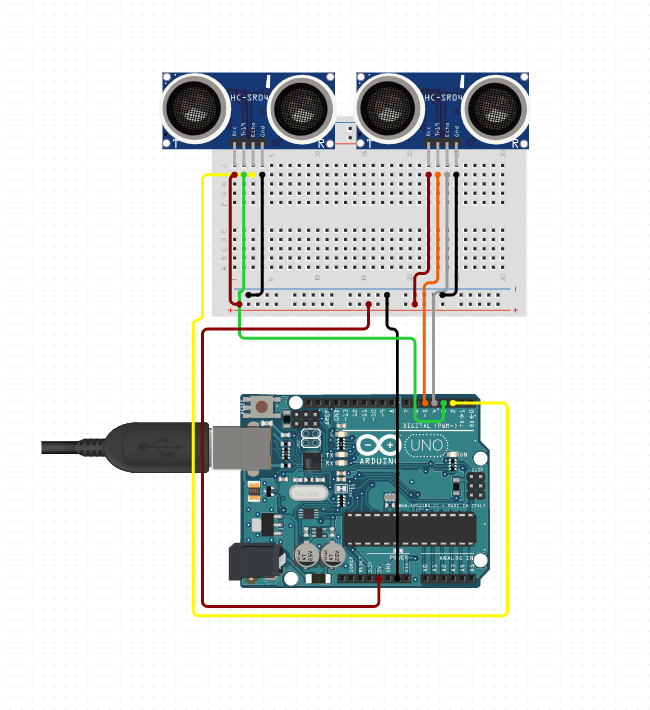
\includegraphics[width=9.35cm]{Arduino Schematics.PNG}}\par
    \caption{An example of how to connect the two sensors to the Arduino}
\end{wrapfigure}

Each sensor covers a different type of notes: the sensor connected to the A0 input, whose position is near to the musician, can play all the white notes in the C3 octave (C3, D3, E3, F3, G3, A3, B3); on the other side, the transceiver connected to the A1 pin, that is placed beyond the first sensor, plays all the black notes in an octave of a keyboard (C3\#, D3\#, F3\#, G3\#, A3\#). 
\\The \textit{MapToNote.ino} file maps all the possible positions of the foot to all the notes of the C3-C4 octave. The messages sent from the Arduino to the serial port are composed by a number, which is the MIDI number of the played note, and a letter: \textit{‘b’} indicates that the note played is black, \textit{‘w’} indicates that the played note is white, and \textit{‘s’} represents the stop note message. A possible sequence of messages could be \textit{“48w”} (C3 note on), \textit{“48s”} (C3 note off), \textit{“54b”} (F3\# note on),  \textit{“54s”} (F3\# note off). All these messages are then mapped in \textit{SuperCollider} and then the info regarding the MIDI note and the gate value (0 when an \textit{‘s’} message is sent, 1 in the other cases) are sent respectively to the \textbf{\textit{$\sim$serialMidiNoteControlBus}} and to the \textbf{\textit{$\sim$serialMidiMessageControlBus}}. The synth then reads from these two buses in order to have the note that has to be played and the gate control, to stop the sound when the sensors don’t see anything. 
\\The black notes sensor has priority to the white notes sensor: in fact, if both the A0 and the A1 sensor see something in their range, the message sent is a \textbf{black note} message. Then, if the black note sensor doesn’t see anything but the white note sensor sees something near, the Arduino sends a \textbf{white note} message. As the last possibility, when the musician is not playing anything placing his foot on the virtual keyboard, the two sensors do not see anything in their range and a \textbf{stop note} message is sent. The Arduino sends a stop note message also when the played note is changed by the musician, changing the foot position on the virtual keyboard. 
\\The maximum ranges set are approximately 20cm for the black note sensor connected to the analog pin A1 and 27cm for the white note sensor connected to the analog pin A0.

\subsection{Wavetable Synthesizer}
The \textbf{Wavetable Synthesizer} aims to create pad-like sounds suitable for background harmony. Basically, wavetable synthesis is a sound synthesis tecnique that is based on periodic reproduction of a \textbf{single-cycle waveform}. Substantially, values representing the single cycle are stored in what is called a \textbf{wavetable} and then read from this data-structure for the signal to be played.
The synth that was developed is a mixture of two different sounds, each one consisting of six partials with different amplitude ratio. This allows to achieve a more complex and interesting timbres. The wavetable synth was implemented through \textit{SuperCollider} language within a \textit{SynthDef} object that also features some effects to be applied on the synth itself. The two wave types that we developed are a \textbf{sinusoidal} wavetable and a \textbf{Chebyshev} wavetable and the sound can be further shaped thanks to the chain of effects and filters that are applied to the final harmonized signal.
\\The synthesizer takes the informations regarding the MIDI note played and the gate control respectively from the \textbf{\textit{$\sim$serialMidiNoteControlBus}} and the \textbf{\textit{$\sim$serialMidiMessageControlBus}}. Then, the output signal of the synthesizer is fed to the \textbf{\textit{$\sim$inputAudioBus}}, which is the input signal of the harmonizer block.

\subsection{HarMMMLonizer}
In order to obtain a rich musical background, we needed something able to turn the selected root note into a chord in tune with the harmony of the song. Therefore we improved and expanded the Harmmmlonizer that we implemented for the first homework.

The new developed features are:
\begin{itemize}
    \item \textbf{Smart pitch ratio computation}: the user has now the opportunity to set the \textbf{key} and the reference \textbf{scale}, and for each voice the \textbf{desired interval} respect to the root note, which we assume to always be the detected one. Fig. \ref{fig:PitchRatioAlg} shows a high-level diagram of the algorithm we have implemented to find the desired pitch ratio in semitones, while Fig. \ref{fig:PitchRatioAlg} shows an example of its application. The algorithm is implemented by the \textbf{pitchRatioManager} \textit{SynhtDef} in \textit{Supercollider}.
    \item \textbf{An optimized pitch shifter} \textit{SynhtDef} that uses the \textit{PitchShiftPA} pseudo-UGen which implements the \textbf{PSOLA} algorithm allowing to maintain the formants while changing the pitch with (particularly useful if the input signal is a human voice).
    \item \textbf{Improved master section}: to the final output signal the user can now apply a \textbf{reverb} with dry/wet, room size and high damp controls, a \textbf{high-pass filter} and a \textbf{low-pass filter} in which the cutoff frequency and the resonance can be modified, a \textbf{Low Frequency Oscillator} modulated by the user in frequency and phase and an \textbf{ADSR envelope}. These effects were implemented in order to give to the user more possibilities to shape the sound. All these parameters are controlled by the user through a more portable and compact GUI created with \textbf{TouchOSC}.
\end{itemize}

\begin{figure}[H]
 \centering
 \subfigure[]{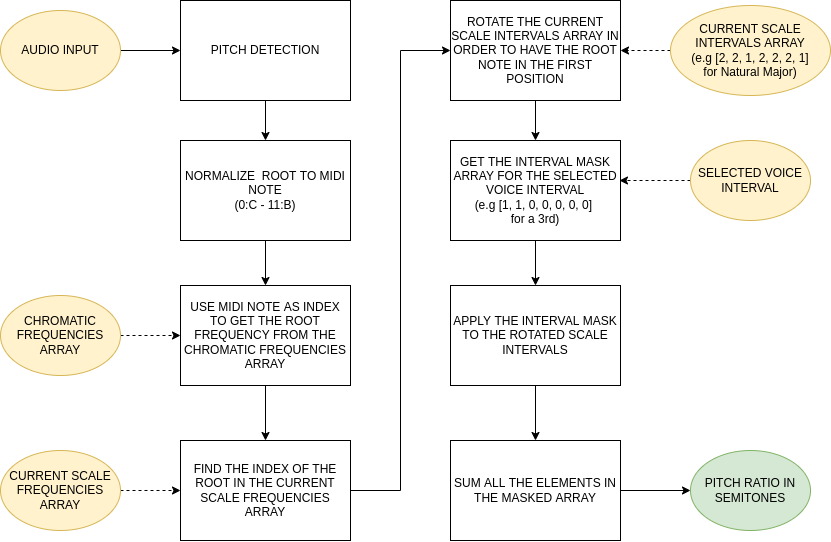
\includegraphics[width=0.50\textwidth]{HarmmmlonizerAlgorithm.png}}
 \hspace{10pt}
 \subfigure[]{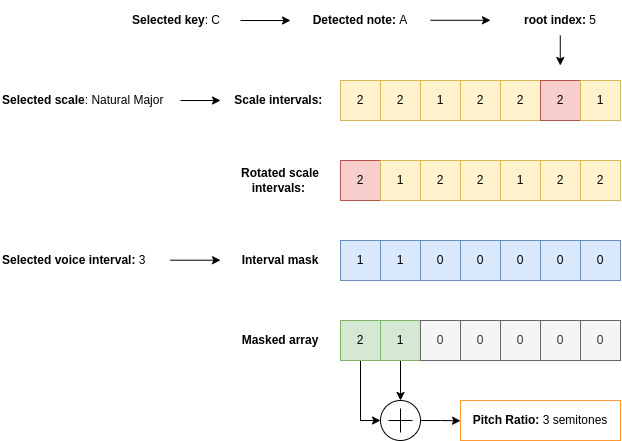
\includegraphics[width=0.50\textwidth]{HarmmlonizerAlgorithmExample.png}} 
 \caption{Harmmmlonizer pitch ratio computation: (a) Algorithm (b) Example}
 \label{fig:PitchRatioAlg}
\end{figure}

\subsection{Graphical User Interface: TouchOSC}

The \textbf{Graphical User Interface (GUI)} was implemented through \textbf{TouchOSC} (Mk1 version), a fully modular control surface that runs on all iOS and Android devices. TouchOSC supports sending and receiving messages through \textbf{OSC (Open Sound Control)} and \textbf{MIDI (Musical Instrument Digital Interface)} protocols. The TouchOSC Editor application allows you to arrange and freely configure all the control elements you need to manage within your GUI. \\
All the graphical elements are contained within what is called a layout. Basically, a layout is a file that contains one or more pages that, in their turn, hold controls element with their individual settings such as OSC-mapping or MIDI-mapping, look and feel configurations and other options in function of the specific element type. Layouts can be transferred to the target device over \textbf{WI-FI network} using TouchOSC Editor app or copied through an USB cable connection. For further information, we recommend visiting TouchOSC Mk1 official website.\\
The layout that was developed consists of three different pages. The first one is devoted to general controls over the final output and the Pitch Shifter. The second page is related to controls over pitched voices, whereas the third one provides controls over Synth Pad parameters. The musician can switch from one page to the other by simply selecting the correct page on the tab-bar section located on top of the screen. Messages are exchanged with the software through OSC communication protocols. Thus, each section within both pages has its own OSC address patterns hierarchy. The Layout was developed for iPad or other tablet devices.


\subsubsection{Page 1: General Controls}

As brought up before, the first page consists of two main sections: \textbf{Master} and \textbf{Pitch Shifter}.

\begin{figure}[H]
\centering
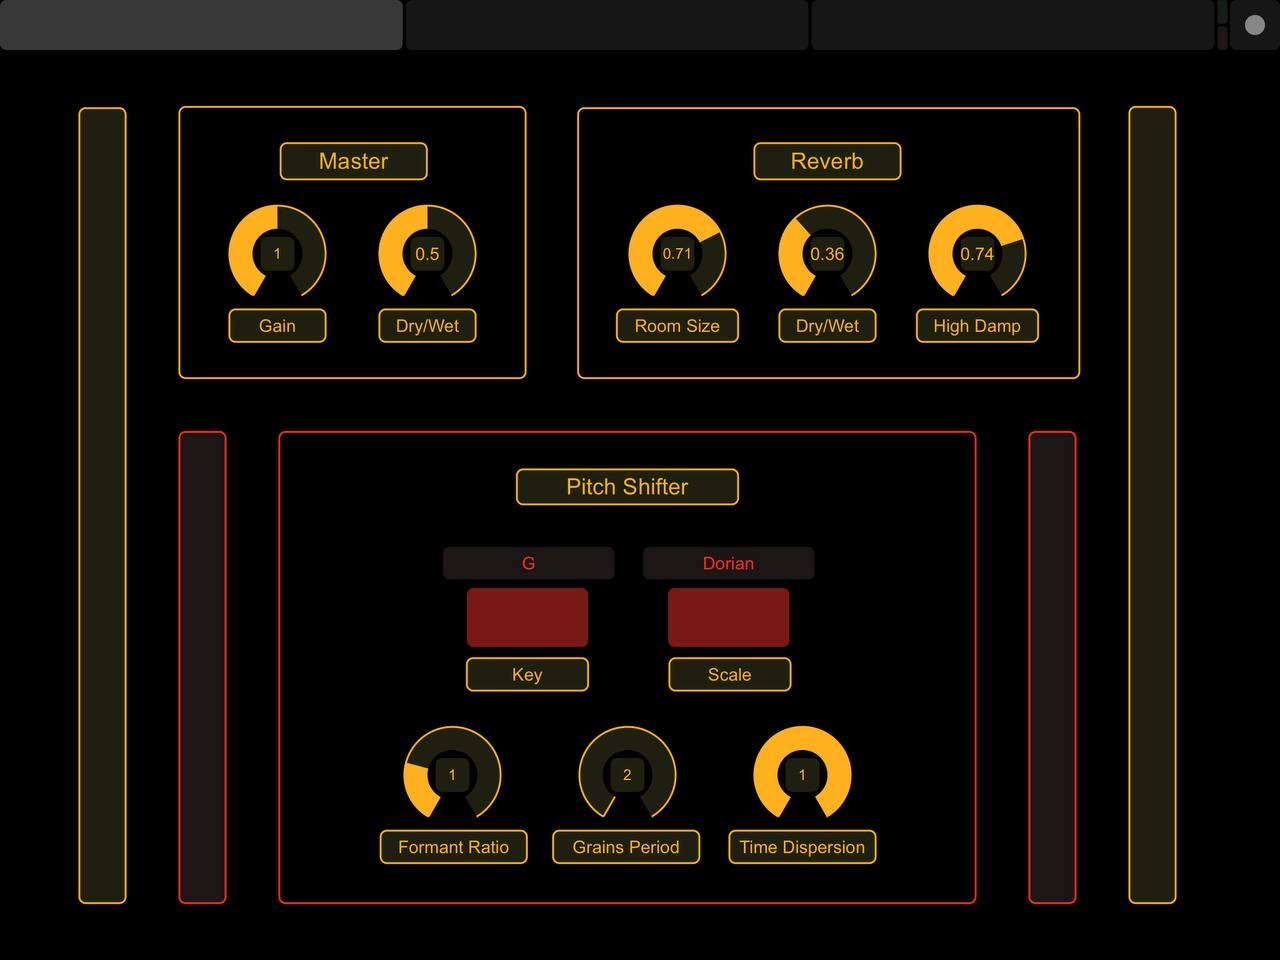
\includegraphics[width=0.65\textwidth]{GeneralControls-TouchOSC-GUI.png}
\caption{General controls page within TouchOSC GUI.}
\label{fig:TouchOSCLayoutPage1}
\end{figure}

The \textbf{Master} section allows the musician to set master gain and dry/wet balance between input signal and pitched voices. Furthermore, some controls over reverberation effect to be accomplished on the final output are provided. Indeed, three knobs are available for Room Size, Dry Wet and High Damp parameters. \\
The \textbf{Pitch Shifter} section makes possible for the artist to set the key and the musical mode for pitch shifting. This controls elements consist of two buttons. By clicking on a button, the user can switch from the current value that is displayed within the corresponding label to next one. Moreover, three knobs are available, each one devoted to a specific parameter related to the pitch shifting. This section enables the musician to set \textbf{Formant Ratio}, \textbf{Grains Period} and \textbf{Time Dispersion}. \\

\subsubsection{Page 2: Pitched Voices Controls}

The \textbf{Voices} pages is divided into four sections, one for each voice, as four voices harmony is supported.

\begin{wrapfigure}{l}{0.65\textwidth}
{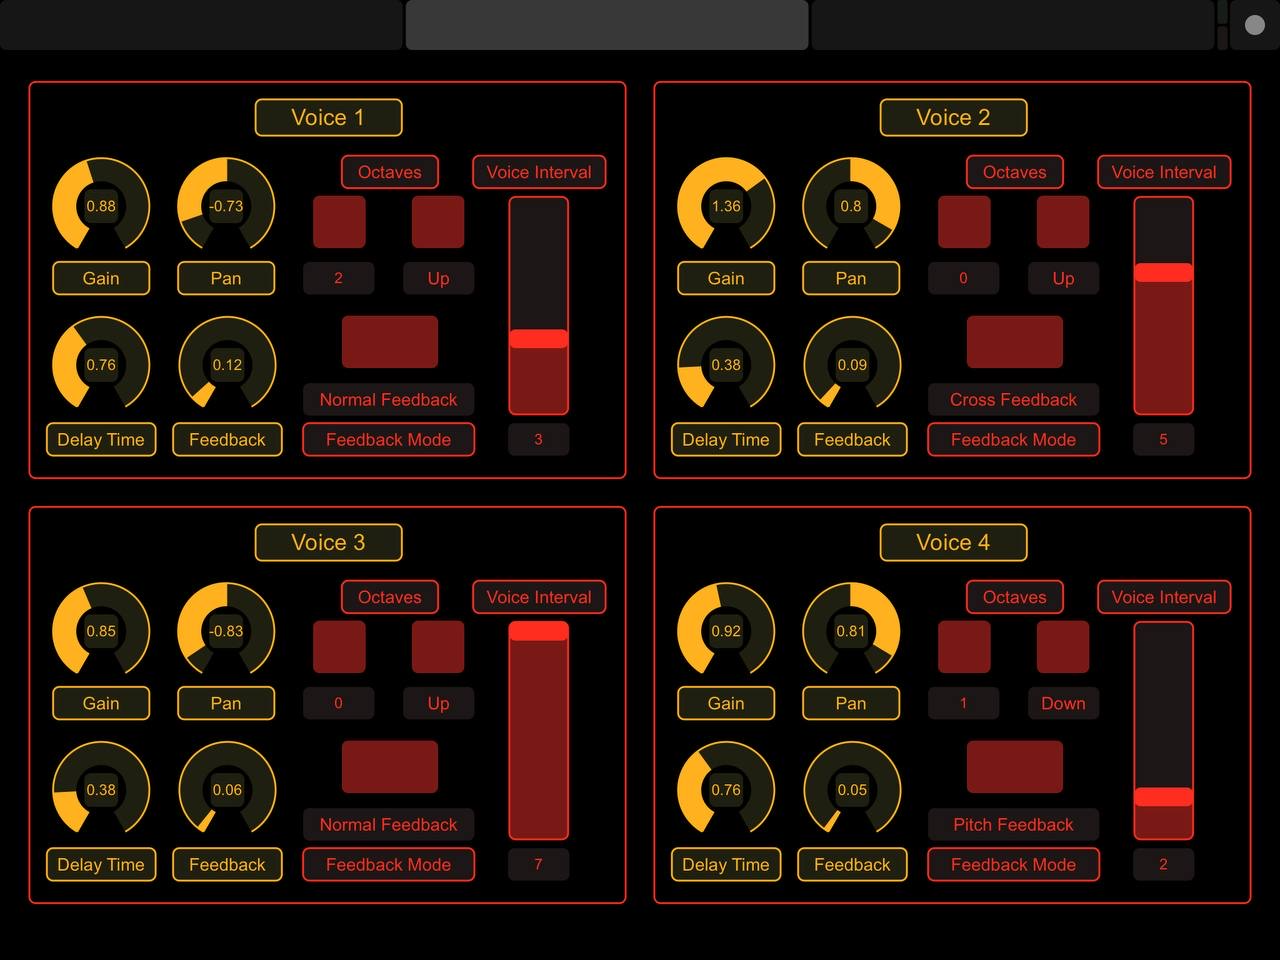
\includegraphics[width=9.35cm]{PitchedVoicesControls-TouchOSC-GUI.png}}\par
    \caption{Pitched voices page within TouchOSC GUI.}
    \label{fig:OSCAddressPatternTouchOSC}
\end{wrapfigure}

For each section, \textbf{Gain} and \textbf{Pan} knobs make possible to set voice gain and panning values. \textbf{Voice Interval} slider allows to set the interval for pitch shifting, whereas the two buttons on its left side enable to set the number of octaves and direction for pitch shifting, which can be accomplished within the same octave as the input note or one/two octaves upward/downward. 

Moreover, some controls over feedback delay line are available. The musician can choose the desired \textbf{Feedback Mode} by clicking on the \textbf{FeedbackMode} button and set \textbf{DelayTime} and \textbf{Feedback amount} values for feedback effect to be applied on the single pitched voice.

\subsubsection{Page 3: Synth Pad Controls}

\begin{wrapfigure}{l}{0.65\textwidth}
{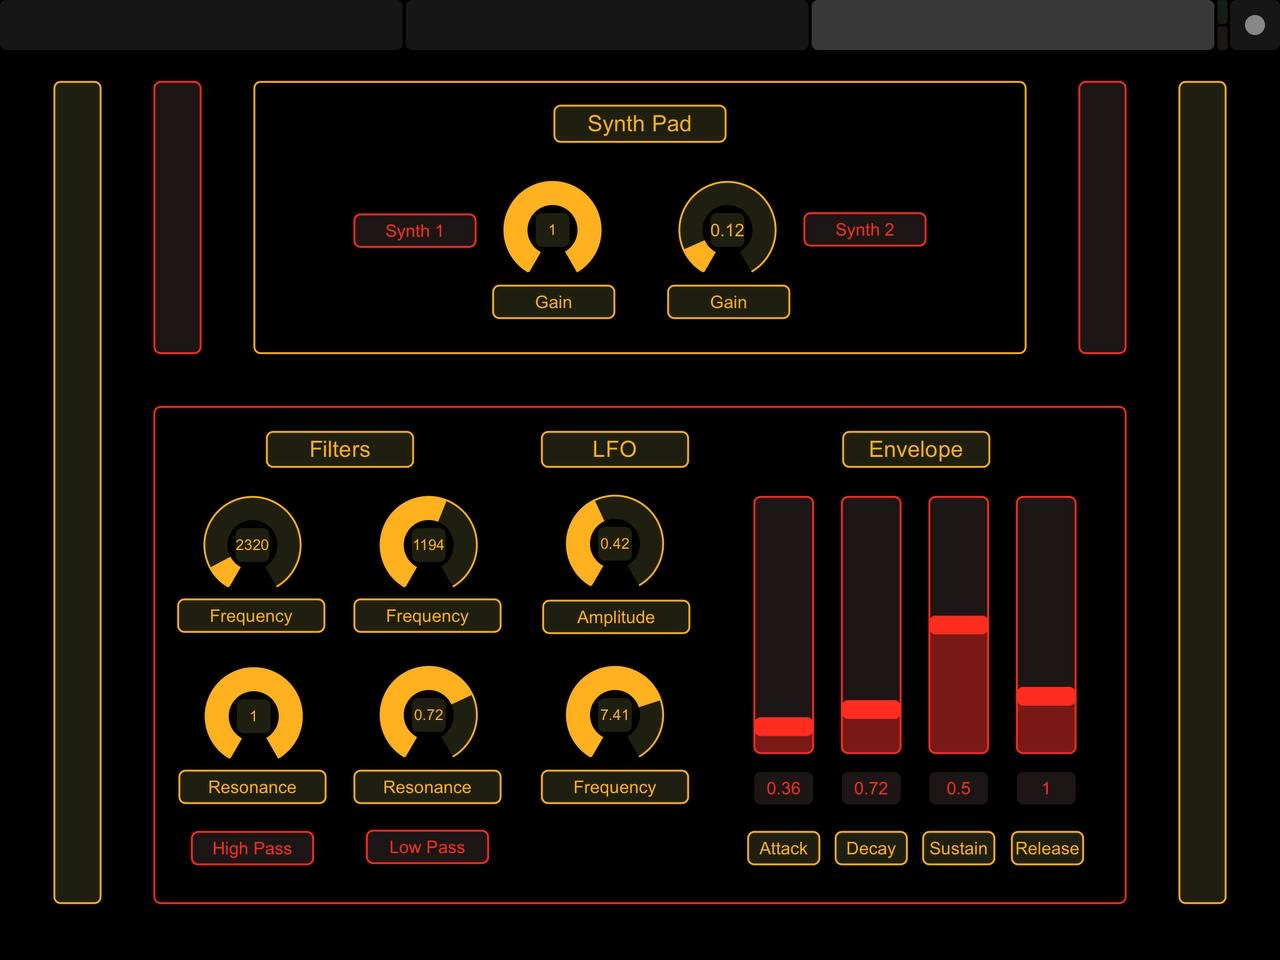
\includegraphics[width=9.35cm]{SynthPadControls-TouchOSC-GUI.png}}\par
    \caption{Synth Pad page within TouchOSC GUI.}
\end{wrapfigure}

The third page is devoted to \textbf{Synth Pad} controls and it consists of two sections.
As the synth pad sound is a mixture of two different sounds, the first section provides the musician with the possibility of controlling the \textbf{balance} between them. Indeed, two gain knobs, one for each synth, are available. \\

The second section makes possible to control parameters related to \textbf{effects} and \textbf{ADSR envelope} to be applied on the synth sound. As a matter of fact, it consists of three subsections. The first one provides controls over \textbf{Frequency} and \textbf{Resonance} of the High Pass and Low Pass filters. Then, two knobs allows the musician to set Amplitude and Frequency of the LFO. Moreover, four sliders are available to control \textbf{Attack}, \textbf{Decay}, \textbf{Sustain} and \textbf{Release} of the ADSR envelope.


\section{Visualization}
\subsection{Introduction}
The visualization is implemented using the \textit{Processing} ability to render rapidly changing shapes and exploiting the Object-Oriented paradigm of Java, upon which the Processing language is based upon. The main idea behind the visualization is to offer a functional graphic section pleasantly integrated with some catchy graphics that could reflect and respond to the user actions.

\begin{figure}[H]
\centering
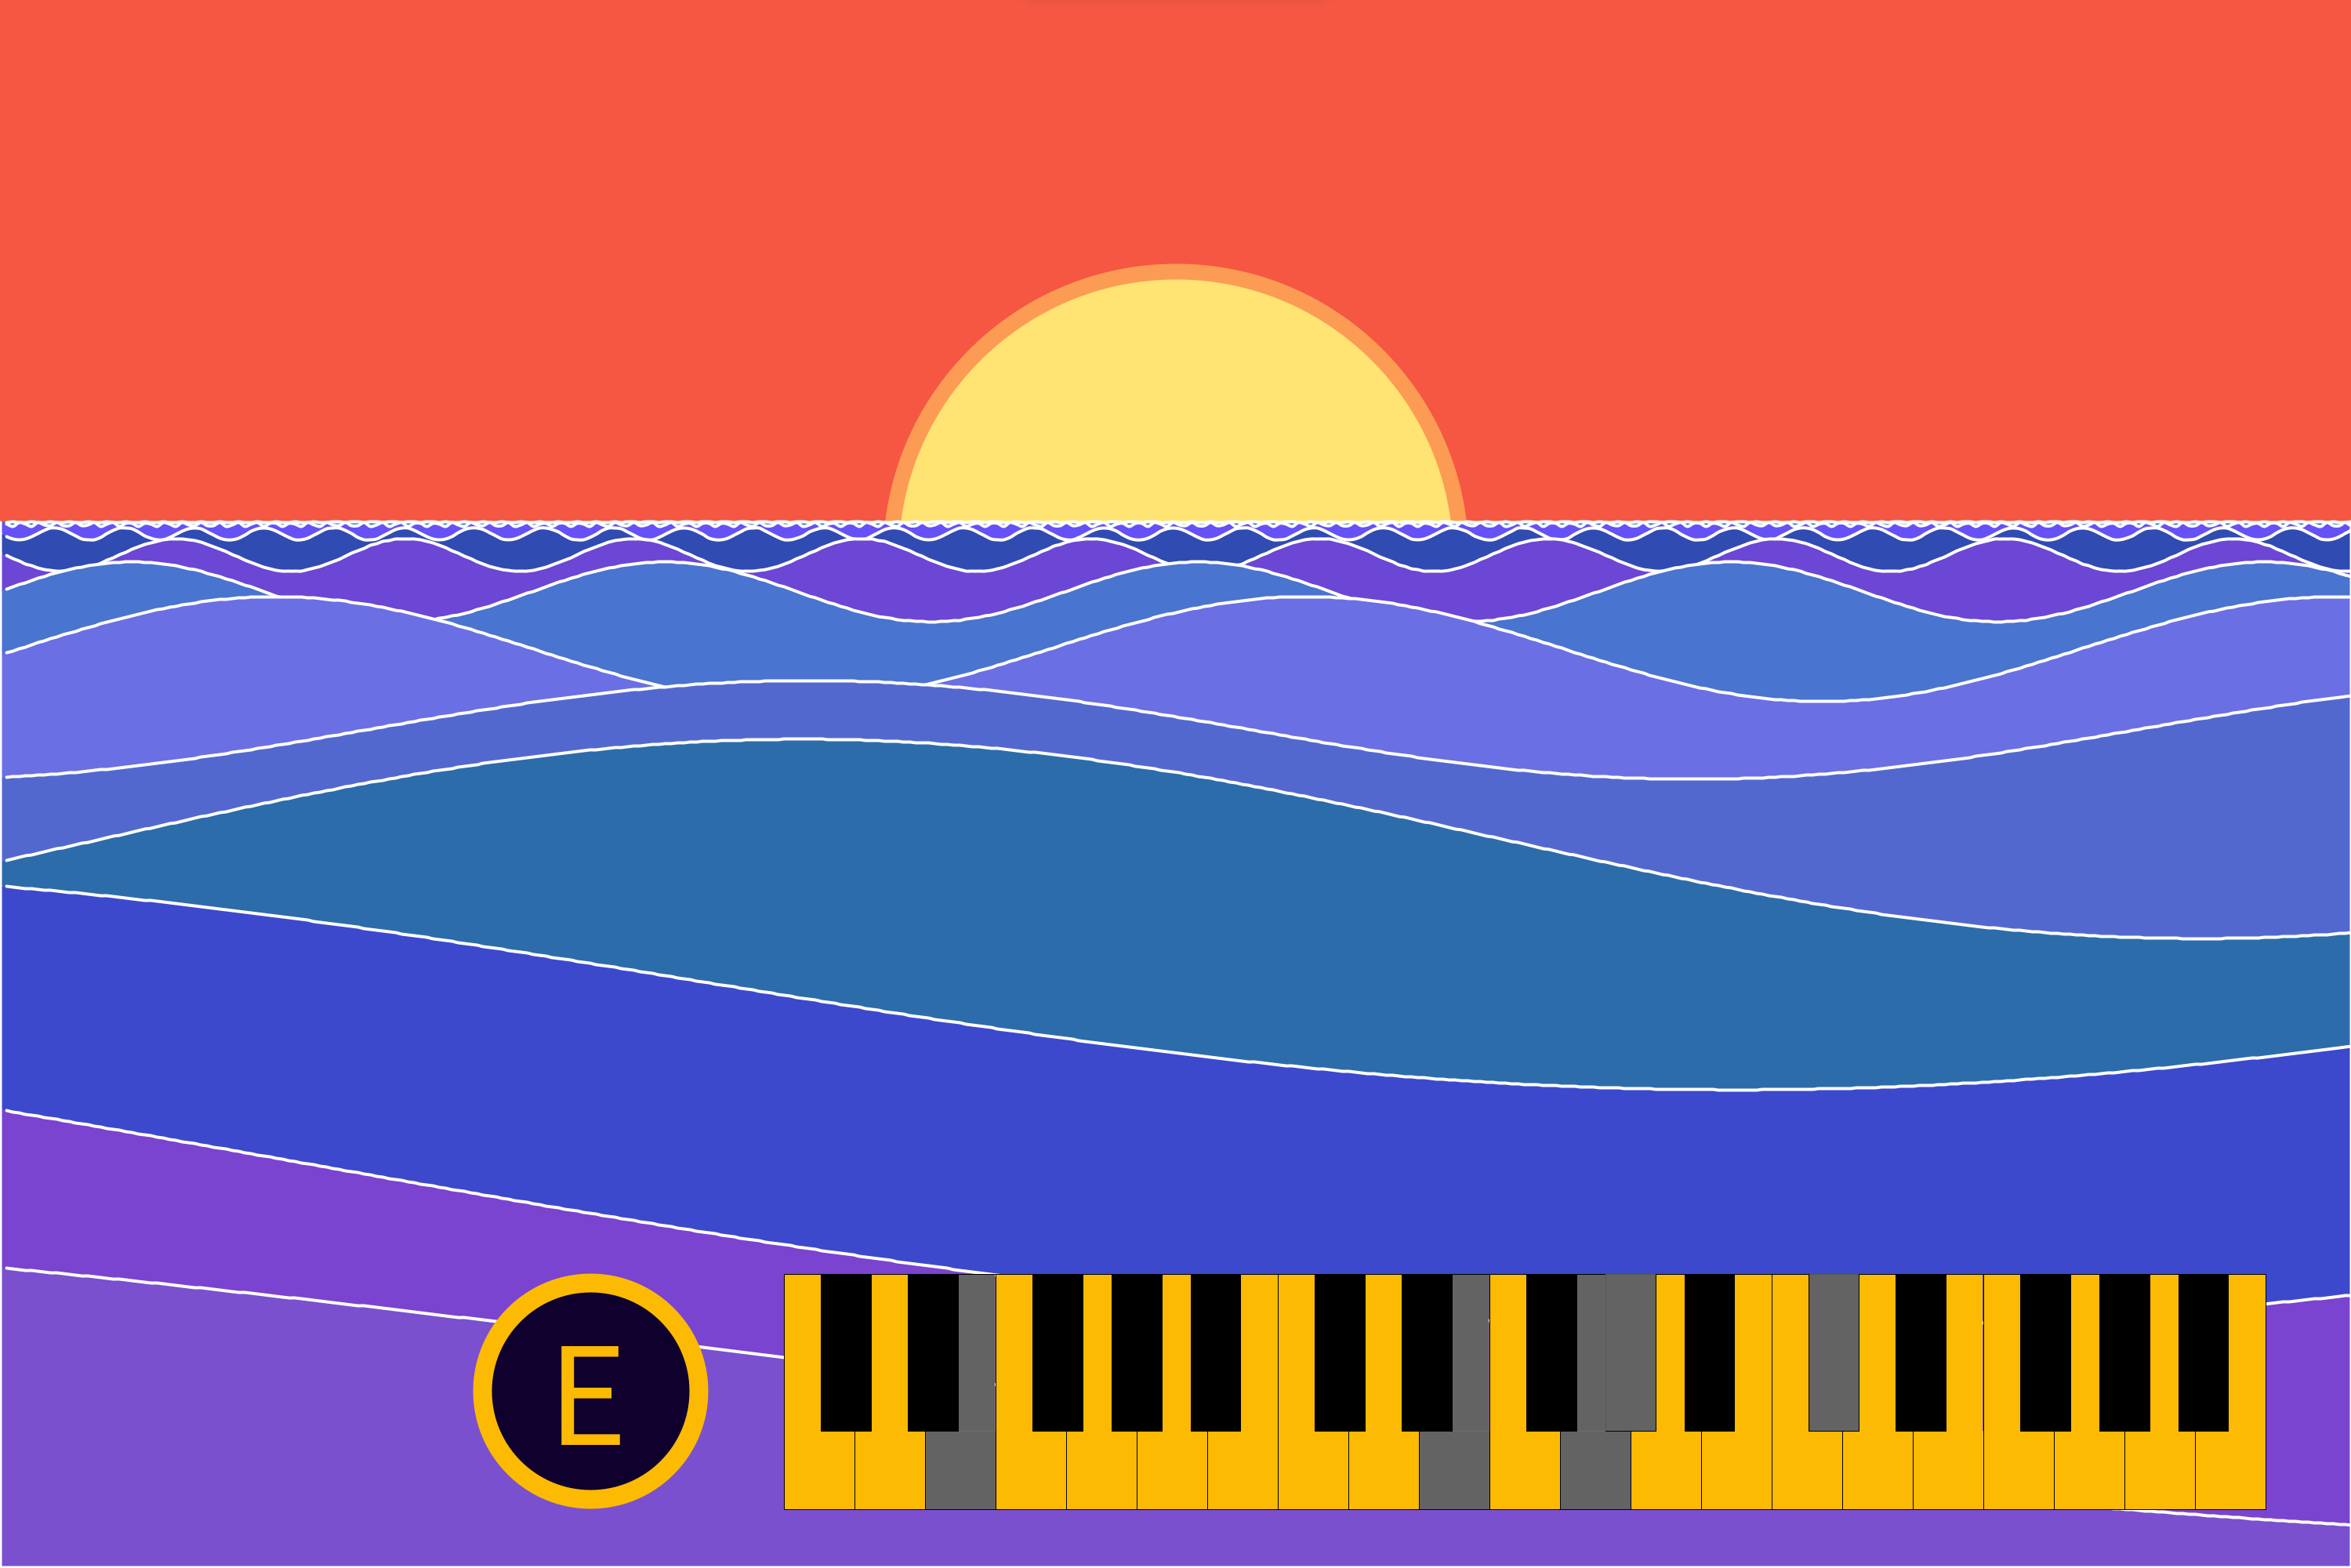
\includegraphics[width=0.8\textwidth]{seaLandscape.png}
\caption{Visualization of the keyboard and animated landscape}
\label{fig:seaLandscape}
\end{figure}

\subsection{Functionalities}
Our project is basically a proof of concept for a highly portable keyboard that could ideally be operated hands-free and autonomously generates chords. Therefore the visualization features a functional block that aims to aid the user to clearly see how the provided tools are operating. On top of that a beautiful landscape that reflects the music produced by the user.\\

The functional block at the bottom of the screen includes:
\begin{itemize}
    \item The \textbf{note} played by the user on the left.
    \item A \textbf{three-octave keyboard} on the right, displaying the root note received from the sensor connected to the Arduino and the generated notes that compose the chord.
\end{itemize}

The animated landscape that reacts to the user’s actions, updating in real time the parameters that define the shape of each element appearing in the picture:

\begin{itemize}
    \item The sun is animated and its radius oscillates between its maximum and minimum set dimension as notes are played.
    \item The waves amplitude, velocity and color palette are updated independently:
    \begin{itemize}
        \item The \textbf{amplitude} is scaled each time a note is played. 
        \item \textbf{Velocity} is increased or slowed down and can even determine a  change of direction of the wave.
        \item The palette that determines the color of each wave in the whole sea is changed accordingly to the \textbf{chord} generated by the harmonizer:
        \begin{itemize}
            \item Major chords generate rgb colors with values of red and blue fixed at 255 and 0 respectively.
            \item Suspended chords generate rgb colors with values of green and blue fixed at 255 and 0 respectively.
            \item Minor Seventh chords generate rgb colors with values of red and green fixed at 0 and 255 respectively.
            \item Minor chords generate rgb colors with values of red and blue fixed at 0 and 255 respectively.
            \item Major Dominant seventh chords generate rgb colors with values of green and blue fixed at 0 and 255 respectively.
            \item Major seventh chords generate rgb colors with values of red and green fixed at 255 and 0 respectively.
            \item Chords with other alterations generate a custom designed palette that includes colors from each other palettes.
        \end{itemize}
        Both colors and chord types are mapped with corresponding moods and feelings that they resemble, as shown in Fig. \ref{fig:ChordColorMoodMapping}. For example, cold colors are associated with unhappy feelings, as minor chords do. Exploiting this, it is possible to create a relation between the chords played by the harmonizer and a color palette. Of course it is to be noted that those relations are subjective.
    \end{itemize}
\end{itemize}

\begin{figure}[H]
\centering
  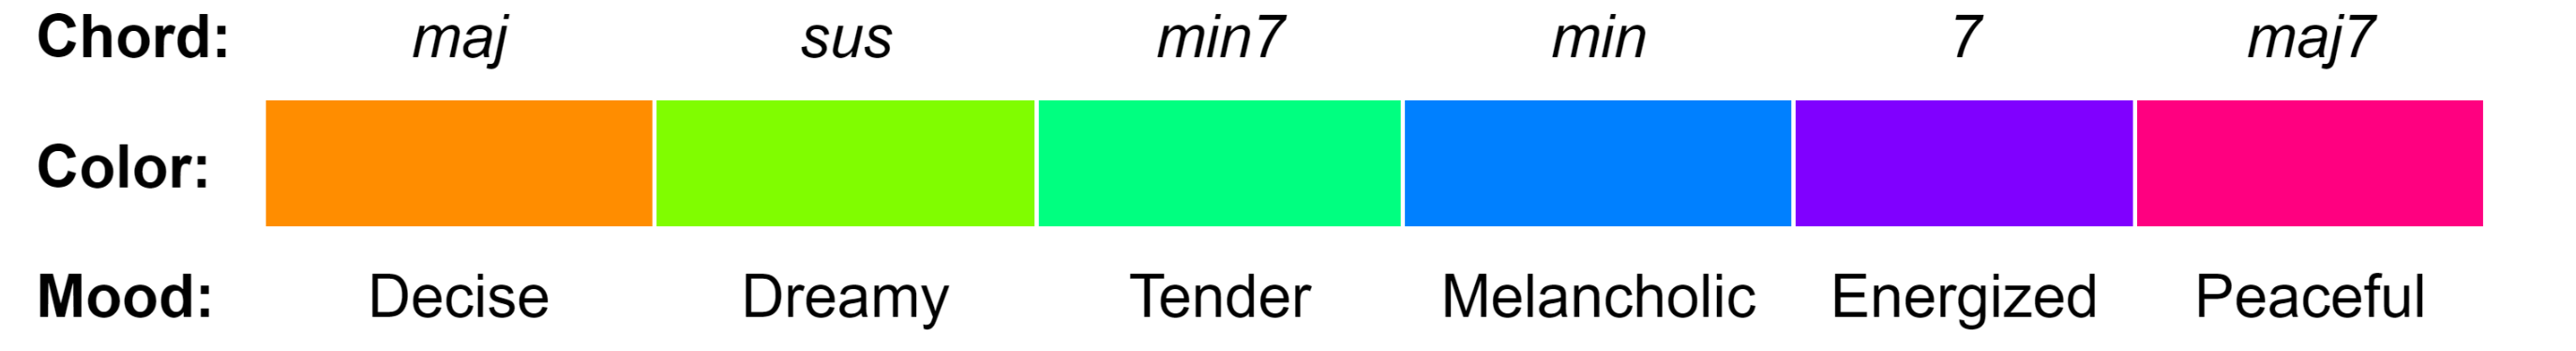
\includegraphics[width=0.85\textwidth]{ChordColorMoodMapping.png}
    \caption{Mapping between chords, mood and colors.}
     \label{fig:ChordColorMoodMapping}
\end{figure}
\vspace{5pt}

\subsection{Connection}
The connection between the visualization and the rest of the system is actuated using OSC messages coming from the harmonizer implemented in \textit{SuperCollider}. \textit{Processing} needs to receive a message that indicates if the user has played a new note or if stopped playing, which root note was selected and the harmonized notes produced by the harmonizer. In order to make this possible, we created an \textit{OscManager} SynthDef that collects the needed data and generates a custom OSC message, with the structure shown in Fig.\ref{fig:OscMessageStructure}.

\begin{figure}[H]
\centering
  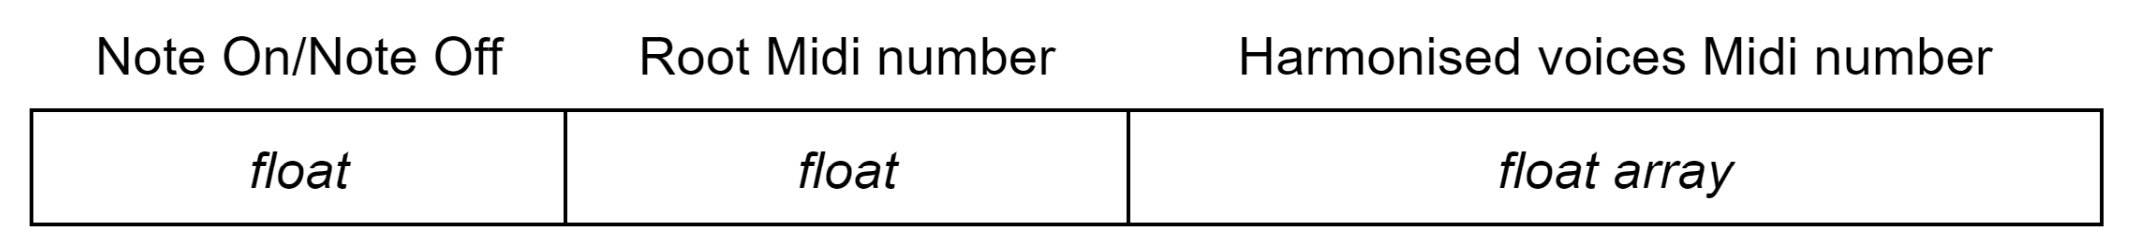
\includegraphics[width=0.85\textwidth]{OscMessageStructure.png}
    \caption{Osc message structure.}
     \label{fig:OscMessageStructure}
\end{figure}
\vspace{5pt}
\section{Conclusions}

On the \textit{Processing} side, the \textit{oscEvent} method provided by \textit{OscP5} and \textit{NetP5} libraries recognizes the incoming OSC message. Once triggered, it creates an event that parses the message using a custom \textit{OscHandler} class and then updates the parameters of the classes generating the keyboard and the landscape.

\subsection{Implementation}
The implementation paradigm follows as much as possible the Object-Oriented paradigm of Java, upon which Processing is based. Therefore we created classes and handlers for each element shown in the landscape to keep the code scalable and intelligible. In order to achieve this we avoided as much as we could explicit calculations inside the \textit{draw} method.\\
The implemented class creates from scratch each element of the visualization. Diving more in detail:
\begin{itemize}
    \item The \textit{RootNameDisplayer} class renders the chord root note name, following the English note convention.
    \item The \textit{PianoKeyboardDisplayer} class renders the keyboard block, allowing to set which notes are currently being played by the user and by the harmonizer.
    \item The \textit{Wave} class creates a single wave and offers methods that change its amplitude, velocity and color.
    \item The \textit{SunHandler} class renders the sun and offers a method that changes its radius.
    \item The \textit{PerspectiveHelper} class has a method that provides the distances used to create a perspective illusion, based on a set vanishing point.
    \item The \textit{ChordBasedColorPicker} class creates a twelve colors palette that changes accordingly to the chord being played.
    \item The \textit{ColorIntepolator} class allows us to interpolate color, creating smooth transitions.
    \item The \textit{ChordRecogniser} class has a method that helps recognize the chord root and chord type being played given the root note and the notes created through the harmonization process.
    \item The \textit{OscHandler} class enables the correct parsing of the incoming Osc messages, which are required to provide the type of incoming message (\textit{NoteOn} or \textit{NoteOff}), the root note and the harmonized notes frequencies.
\end{itemize}

\subsection{Results}
The final result of our project is a prototype for a highly portable tool that could help musicians to enrich their live sets, in particular in situations where a solid harmonic base is needed as happens in semi-acoustic sets. Nevertheless it is to remember that what we produced is still a proof of concept. For example, with better performing sensors we could afford to use a larger keyboard, easily improving the usability of the instrument. 

\subsection{Future Improvements}

As a future improvement, we could use other kind of sensors connected to Arduino to increase the maximum range of each group of notes.
\\ Regarding the harMMMLonizer at the moment only heptatonic scales are supported but it will be nice to add pentatonic, hexatonic and octatonic scales support as well.
\\Another idea of possible improvement is to connect an external device different from the TouchOSC application to change the parameters of the synthesizer and the harMMMLonizer. For example, connecting a joypad could be another smart and convenient way to modulate the parameters of our computer music system.
\\On the design part, we had the idea to build a wooden keyboard instead of using simple paper. Even if this choose makes our project less easily portable, it could be a good add for the use at home of our computer music system.

\end{document}

